\section{Experiment Definition}\label{sec:definition}

Following the Goal--Question--Metric template \cite{wohlin12}, the goal of this experiment is:

\begin{quote}
\textbf{Analyze} self-hosted LLM proposer architectures and agent-loop configurations\\
\textbf{for the purpose of} evaluation\\
\textbf{with respect to} their energy efficiency and task accuracy\\
\textbf{from the point of view of} researchers and practitioners who want to self-host LLMs\\
\textbf{in the context of} the \texttt{autoresearch} agentic AutoML loop running on self-hosted (GPU and CPU-only) hardware.
\end{quote}

The goal refines into two research questions:

\begin{description}[leftmargin=1.2em]
\item[RQ1.] \emph{How do agent-loop configuration choices move the energy/accuracy profile of \texttt{autoresearch}?}
\item[RQ2.] \emph{Which configurations sit on the energy/accuracy Pareto frontier?}
\end{description}

RQ1 is analytic: it quantifies the main and interaction effects of proposer architecture, patience, and loop budget on session energy and final accuracy, together with the mechanistic decomposition (proposer vs.\ training energy, energy wasted on reverted mutations). RQ2 is synthetic: it aggregates the same measurements into a Pareto frontier over (total session energy, final accuracy) and reads off the non-dominated configurations, including the designated baseline cell against which improvements are reported. The CPU-only phase re-evaluates a subset of frontier cells to test whether the frontier survives GPU-less proposer serving.

\begin{figure}[htbp]
\centering
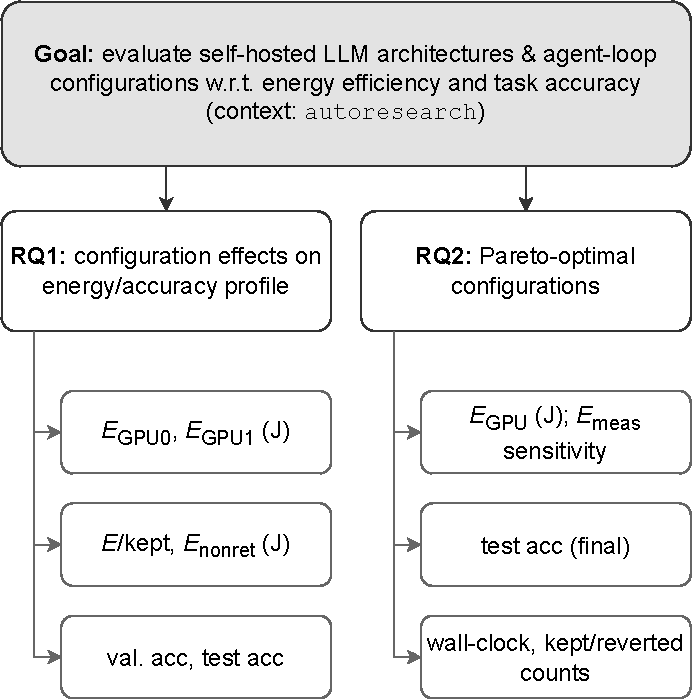
\includegraphics[width=\columnwidth]{figures/gqm.drawio.pdf}
\caption{GQM tree: goal, research questions, and metrics.}
\label{fig:gqm}
\end{figure}

Figure~\ref{fig:gqm} maps the goal to questions and metrics. All energy metrics are direct measurements (RAPL/NVML via \texttt{EnergiBridge}); accuracy metrics are ground-truth workload outcomes (validation accuracy during the loop and CIFAR-10 test-set accuracy at session end), deliberately distinct from the agent's own keep/revert judgments, which this experiment treats as behavioral signals rather than accuracy measures.
